\begin{figure*}[ht!]
\begin{center}% note that \centering uses less vspace...
\resizebox{2\columnwidth}{!}{%
\begin{tabular}{lllll}


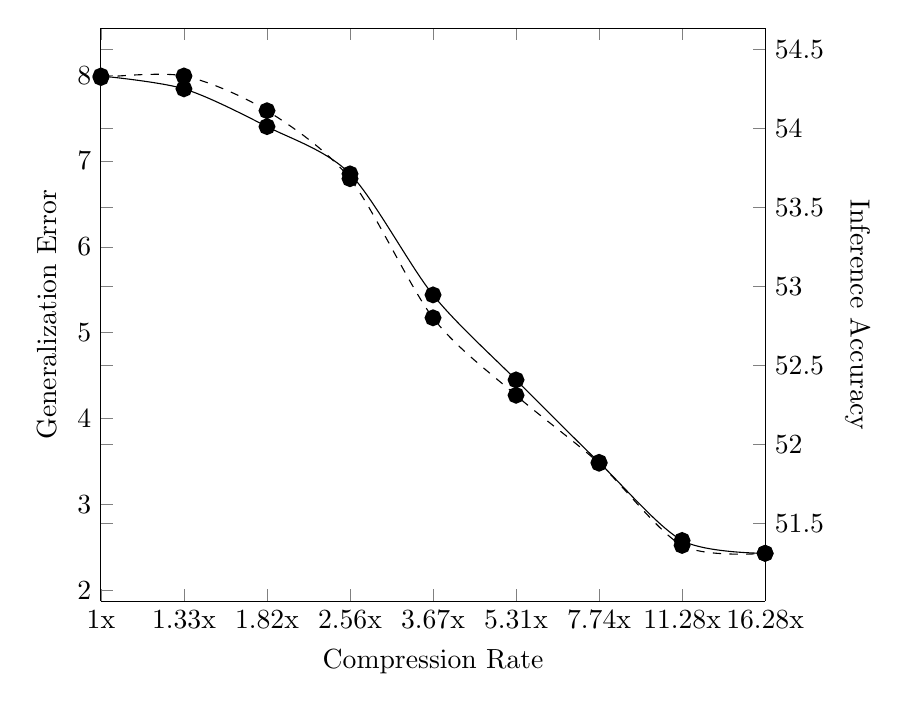
\begin{tikzpicture}
% let both axes use the same layers
\pgfplotsset{set layers}
%
\begin{axis}[
scale only axis,
line width=2.0pt,
mark size=2.0pt,
xmin=0,xmax=8,
ylabel={Generalization Error},
axis y line*=left,
xlabel={Compression Rate},
xtick={0,1,2,3,4,5,6,7,8},
xticklabels={1x, 1.33x, 1.82x, 2.56x, 3.67x, 5.31x, 7.74x, 11.28x, 16.28x}
]
\addplot[
    color=black,
    solid,
    mark=*,
    mark options={solid},
    smooth
    ]
    coordinates {
    (0,7.99)(1,7.84)(2,7.4)(3,6.85)(4,5.44)(5,4.45)(6,3.49)(7,2.58)(8,2.43)
      };
\end{axis}

\begin{axis}[
scale only axis,
line width=2.0pt,
mark size=2.0pt,
xmin=0,xmax=8,
ylabel near ticks, yticklabel pos=right,
ylabel={Inference Accuracy},
ylabel style = {rotate=180},
axis x line=none
]
\addplot[
    color=black,
    dashed,
    mark=*,
    mark options={solid},
    smooth
    ]
    coordinates {
    (0,54.32)(1,54.33)(2,54.11)(3,53.68)(4,52.80)(5,52.31)(6,51.88)(7,51.36)(8,51.31)
        };
\end{axis}
\end{tikzpicture} &

%
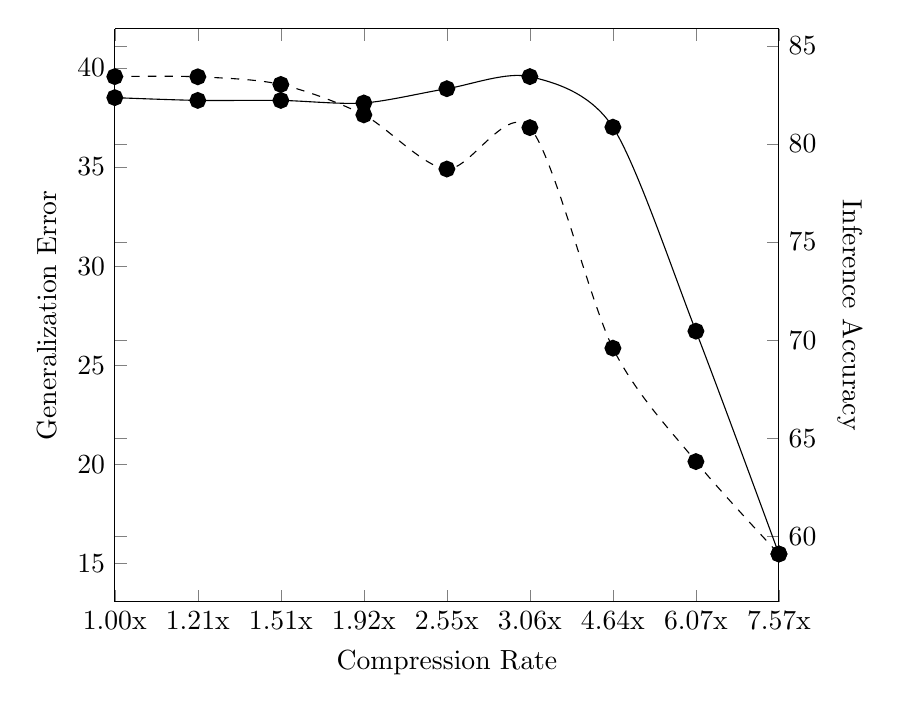
\begin{tikzpicture}
% let both axes use the same layers
\pgfplotsset{set layers}
%
\begin{axis}[
scale only axis,
line width=2.0pt,
mark size=2.0pt,
xmin=0,xmax=8,
ylabel={Generalization Error},
axis y line*=left,
xlabel={Compression Rate},
xtick={0,1,2,3,4,5,6,7,8},
xticklabels={1.00x, 1.21x, 1.51x, 1.92x, 2.55x, 3.06x, 4.64x, 6.07x, 7.57x}
]
\addplot[
    color=black,
    solid,
    mark=*,
    mark options={solid},
    smooth
    ]
    coordinates {
    (0,38.5)(1,38.36)(2,38.36)(3,38.23)(4,38.95)(5,39.56)(6,37.01)(7,26.72)(8,15.48)
      };
\end{axis}

\begin{axis}[
scale only axis,
line width=2.0pt,
mark size=2.0pt,
xmin=0,xmax=8,
ylabel near ticks, yticklabel pos=right,
ylabel={Inference Accuracy},
ylabel style = {rotate=180},
axis x line=none
]
\addplot[
    color=black,
    dashed,
    mark=*,
    mark options={solid},
    smooth
    ]
    coordinates {
    (0,83.43)(1,83.42)(2,83.03)(3,81.48)(4,78.72)(5,80.83)(6,69.59)(7,63.81)(8,59.10)
        };
\end{axis}
\end{tikzpicture} &





%
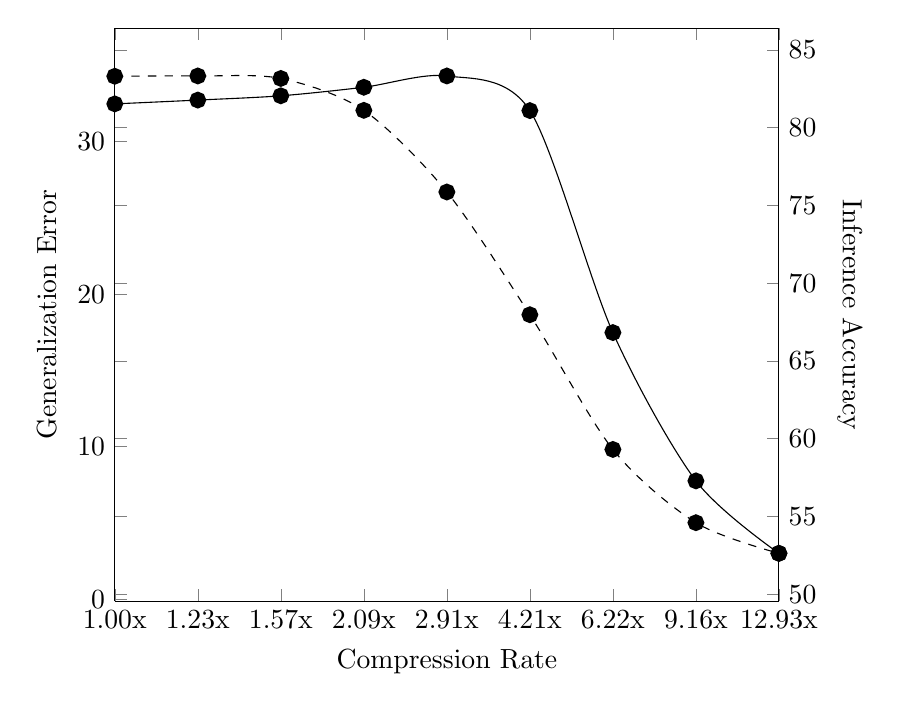
\begin{tikzpicture}
% let both axes use the same layers
\pgfplotsset{set layers}
%
\begin{axis}[
scale only axis,
line width=2.0pt,
mark size=2.0pt,
xmin=0,xmax=8,
ylabel={Generalization Error},
axis y line*=left,
xlabel={Compression Rate},
xtick={0,1,2,3,4,5,6,7,8},
xticklabels={1.00x, 1.23x, 1.57x, 2.09x, 2.91x, 4.21x, 6.22x, 9.16x, 12.93x}
]
\addplot[
    color=black,
    solid,
    mark=*,
    mark options={solid},
    smooth
    ]
    coordinates {
    (0,32.47)(1,32.72)(2,33)(3,33.56)(4,34.3)(5,32.03)(6,17.48)(7,7.76)(8,3.01)
      };
\end{axis}

\begin{axis}[
scale only axis,
line width=2.0pt,
mark size=2.0pt,
xmin=0,xmax=8,
ylabel near ticks, yticklabel pos=right,
ylabel={Inference Accuracy},
ylabel style = {rotate=180},
axis x line=none
]
\addplot[
    color=black,
    dashed,
    mark=*,
    mark options={solid},
    smooth
    ]
    coordinates {
    (0,83.30)(1,83.32)(2,83.16)(3,81.11)(4,75.86)(5,67.97)(6,59.31)(7,54.60)(8,52.63)
        };
\end{axis}
\end{tikzpicture}


\end{tabular}
}
\caption{\underline{Pruning reduces Inference Accuracy at the cost of Prediction Accuracy.} On pruning the models trained on FashionMNIST(left), Purchase100(Center) and Location(Right) dataset, we find that the inference accuracy decreases (dashed line) due to the decrease in the generalisaton error (solid) and lower prediction accuracy.}
\label{fig:prune}
\end{center}
\end{figure*}
